The new maps or levels encourage gamers to explore the game in a variety of terrains. The addition of aliens made the game more difficult, and this feature also permitted the addition of laser weapons. The alien's movement is implemented using the same mechanism as the platforms provided in the skeleton code. With a few changes, the shooting functionality was also easily implemented utilizing the pre-existing struct. Because having infinite weapon ammo would make the game easy, I set a restriction to how much it can be used by utilizing a counter and only allowing one hundred bullets when the player spawns, however, the player earns more bullets when orbs are gathered.

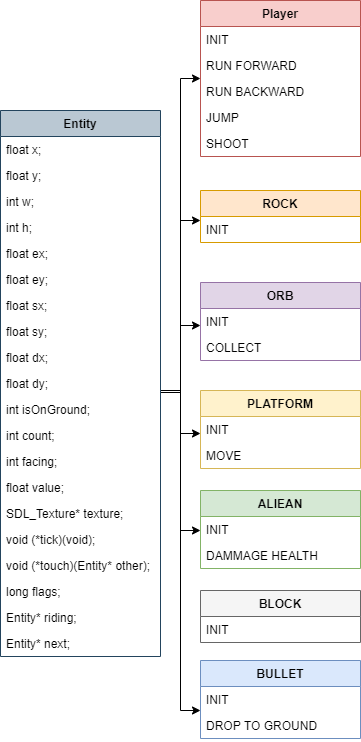
\includegraphics[width=.35\linewidth]{images/UML.png}
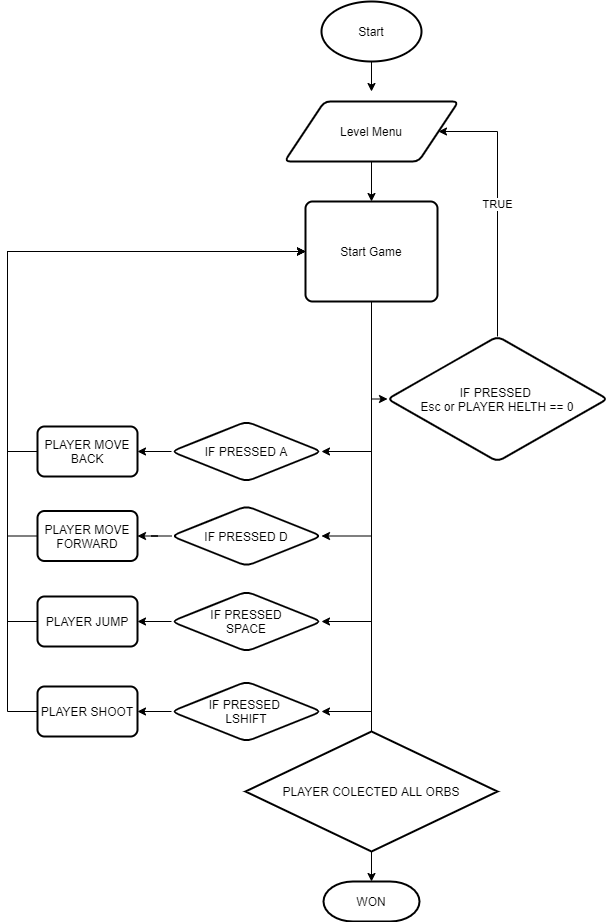
\includegraphics[width=.45\linewidth]{images/top-level.png}

The controls to the player are listened for in the game loop once the game starts. To interact with the game, the user can then move, shoot, or jump using W A S D Right Shift or spacebar. If the player gathers all of the orbs on the map, the game finishes, and the level is completed. If the player touches the alien, it loses health, and if it falls below zero, the game terminates, and the player is returned to the menu. This is visualized using the flowchart below.
